%%%%%%%%%%%%%%%%%%%%%%%%%%%%%%%%%%%%%%%%%%%%%%%%%%%%%%%%%%%%%%%
%
% 		Dissertation template
%
%%%%%%%%%%%%%%%%%%%%%%%%%%%%%%%%%%%%%%%%%%%%%%%%%%%%%%%%%%%%%%%
\documentclass[a4paper, 12pt]{report}

\usepackage{import}
\usepackage{Utilities/utilities}

 

\newacronym{snn}{SNN}{Spiking Neural Networks}
\newacronym{ann}{ANN}{Artificial Neural Networks}
\newacronym{dnn}{DNN}{Deep Neural Networks}
\newacronym{dl}{DL}{Deep Learning}

\newacronym{nn}{NN}{Neural Networks}
\newacronym{ai}{AI}{Artificial Intelligence}
\newacronym{ml}{ML}{Machine Learning}

\newacronym{rl}{RL}{Reinforcement Learning}
\newacronym{dqn}{DQN}{Deep Q-network}
\newacronym{stdp}{STDP}{Spike-Time Dependent Plasticity}
\newacronym{ltp}{LTP}{Long-Term Potentiation}
\newacronym{ltd}{LTD}{Long-Term Depression}
\newacronym{psp}{PSP}{Postsynaptic Potentiation}
\newacronym{epsp}{EPSP}{Excitatory Postsynaptic Potentiation}
\newacronym{ipsp}{IPSP}{Inhibitory Postsynaptic Potentiation}

\newacronym{bmi}{BMI}{Brain Machine Interface}
\newacronym{bci}{BCI}{Brain Computer Interface}
\newacronym{ssp}{SSP}{Structural Synaptic Plasticity}
\newacronym{cnn}{CNN}{Convolutional Neural Networks}
\newacronym{rnn}{RNN}{Recurrent Neural Networks}

\newacronym{lif}{LIF}{Leaky-Integrate Fire}
\newacronym{hh}{HH}{Hodgkin Huxley}

\newacronym{tcga}{TCGA}{The Cancer Genome Atlas Program}

\newacronym{ea}{EA}{Evolutionary Algorithms}
\newacronym{es}{ES}{Evolutionary Strategies}
\newacronym{ga}{GA}{Genetic Algorithms}
\newacronym{cgp}{CGP}{Cartesian Genetic Programming}

\newacronym{pca}{PCA}{Principal Component Analysis}
\newacronym{nmf}{NMF}{Non-matrix factorisation}
\newacronym{umap}{UMAP}{Uniform Manifold Approximation and Projection}
\newacronym{tsne}{t-SNE}{t-Distributed Stochastic Neighbor Embedding}
\newacronym{ge}{GE}{Gene Expression}
\newacronym{mibc}{MIBC}{Muscle Invasive Bladder Cancer}

\newacronym{jbu}{JBU}{Jack Birch Unit}


% define line-spacing
% \linespread{1.25}

% \renewcommand{\familydefault}{\sfdefault}
% \geometry{left=3cm,right=3cm,top=2cm,bottom=2cm}

% % % for proof read
% \linespread{1.75}

\begin{document}

\import{Utilities/}{title.tex}


%%%%%%%%%%% Table of Contents, Figures and Images %%%%%%%%%%% 

\setcounter{tocdepth}{4}
% \setcounter{tocdepth}{5}


%this needs to be defined before inserting the table of contents
% \setcounter{tocdepth}{1} % Show sections
% \setcounter{tocdepth}{2} % + subsections
% \setcounter{tocdepth}{3} % + subsubsections
% \setcounter{tocdepth}{4} % + paragraphs
% \setcounter{tocdepth}{5} % + subparagraphs


\pagenumbering{Roman}

\import{Sections/}{abstract.tex}
\import{Sections/}{acknowledgments.tex}


\tableofcontents
\newpage

\listoffigures
\newpage

\listoftables
% \listoflistings

% \printglossary[type=acronym,style=long,nonumberlist]
\clearpage


\printglossary[nonumberlist]

\printglossary[type=\acronymtype,nonumberlist]
\newpage

\pagenumbering{arabic}
% \newpage



\import{Sections/}{intro.tex}

% \import{Sections/Lit_review/}{master.tex}
\import{Sections/ClusteringAnalysis/}{master.tex}


% \import{Sections/Network_I/}{master.tex}


% \newpage
% \newgeometry{left=1.5cm, right=1.5cm, top=0.5cm, bottom=1cm}
% \begin{figure}[p]
%   \thispagestyle{empty} % Suppress the page number on this page
%   \centering
%   \captionsetup{justification=centering, labelfont=bf}
%     \parbox{\textwidth}{\centering \Huge Tumour derived Network - SBM} % 
%   \vspace{3cm} 
%   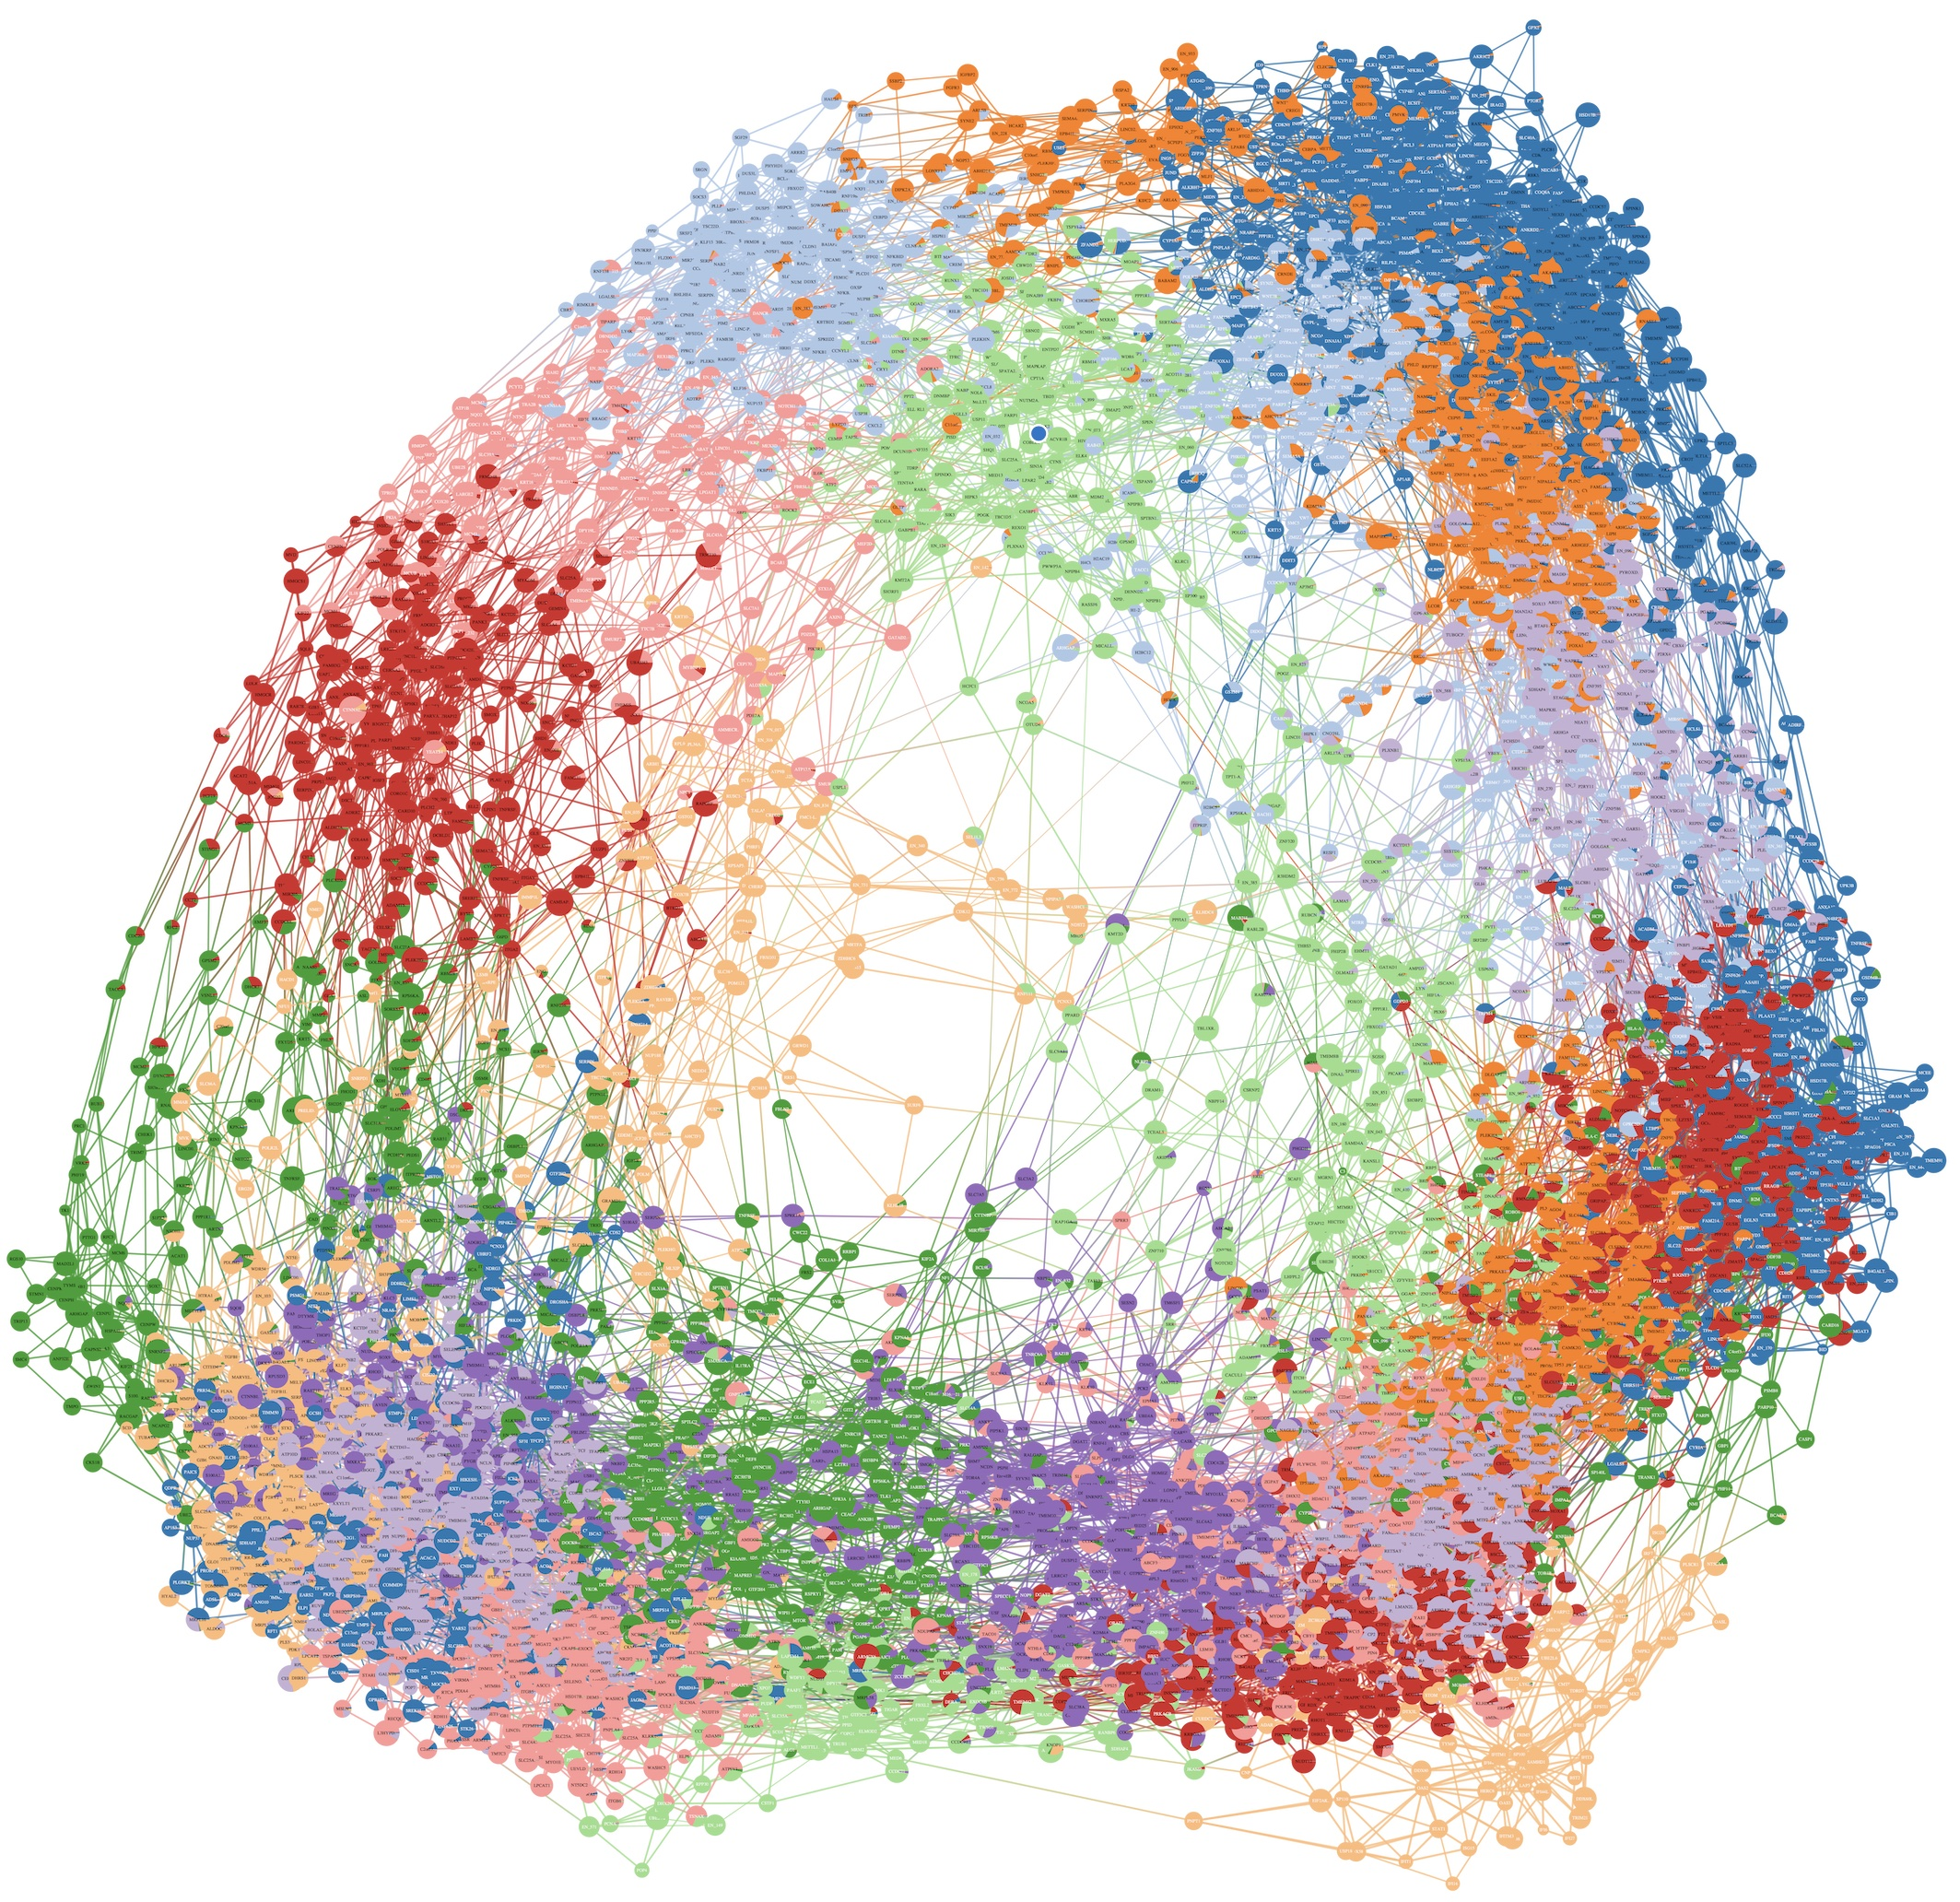
\includegraphics[width=0.9\paperwidth, height=0.9\paperheight, keepaspectratio]{Sections/Network_I/Resources/networks/sbm_standard_5K_6TF_lowRes.png} % Full-page image
%   \parbox{0.8\textwidth}{\centering Network created from using the 5000 most varied genes in the tumour dataset, no weight modifier, minimum degree of 3 for standard genes and 6 for TF.}
% \end{figure}
% \restoregeometry
% \newpage

% \import{Sections/Network_I/EdgePruning}{master.tex}


% \import{Sections/Network_II/}{master.tex}

\import{Sections/}{discussion.tex}


\chapter{Ethics statement}

There was no new data generated in this study and all the gene expression, mutational data was taken from existing resources.

Access to raw RNA sequencing data from TCGA's MIBC cohort was granted through Dr Andrew Mason's dbGaP project \#25297 and processed on The University of York's High Performance Computing Clusters Viking and Viking2, in accordance with local and eRA data processing policies.

Data for the Urotheliome project was generated by RNAseq from human urothelium either freshly isolated for in situ analysis (P0) or following cell culture. The tissues were collected at surgery with the following National Health Service (NHS) Research Ethics Committee (REC) approvals

\begin{itemize}
    \item REC reference: 99/095. "Use of excess ureter from transplant donor kidneys for research purposes". Leeds (East) Research Ethics Committee (latest annual report approved May 2023). These samples were collected as surgical waste and processed anonymously.
    \item REC reference: 21/YH/0225. "URoBank: Urothelial Research Tissue Bank (Phase 2)". Leeds (East) Research Ethics Committee (latest annual report approved Nov 2023). These samples were collected with consent and used anonymously either linked or unlinked to clinical records.  
\end{itemize}

Upon receipt, samples were ascribed a unique "Y" number (eg Y1423) during processing to separate the urothelial cells for RNAseq ("P0") and/or NHU cell culture.

\import{Sections/}{appendix.tex}


%%%%%%%% not include in the PhD %%%%%%%%
% \import{Sections/Gene_Sel/}{master.tex}
% \import{Sections/Miscellanious/}{master.tex}



\bibliographystyle{IEEEtranN}
\bibliography{paperpile}


\end{document}

